\section{Versuchsaufbau und Durchführung}
\subsection{Aufgabe 1: Diagramme der Komponenten}
\section*{Beschreibung des Messsystems}
Das EKG-Messsystem basiert auf einem SparkFun RedBoard zur Datenerfassung und -verarbeitung. Die Herzaktivität wird über Elektroden aufgenommen, durch ein Sensormodul aufbereitet und anschließend über eine serielle Schnittstelle an einen PC zur Visualisierung übertragen. Die nachfolgenden Tabellen beschreiben die wesentlichen Komponenten sowie die verwendeten Signalpfade und Kommunikationsbussysteme, welche die Grundlage für die zu erstellenden Diagramme bilden.

\begin{figure}[H]
    \centering
    \includegraphics[width=1\textwidth]{figures/Messsystem.jpg}
    \caption{Blockschaltbild des EKG-Messsystems mit Signalfluss von links nach rechts.}
    \label{fig:blockschaltbild}
\end{figure}

\begin{figure}[H]
    \centering
    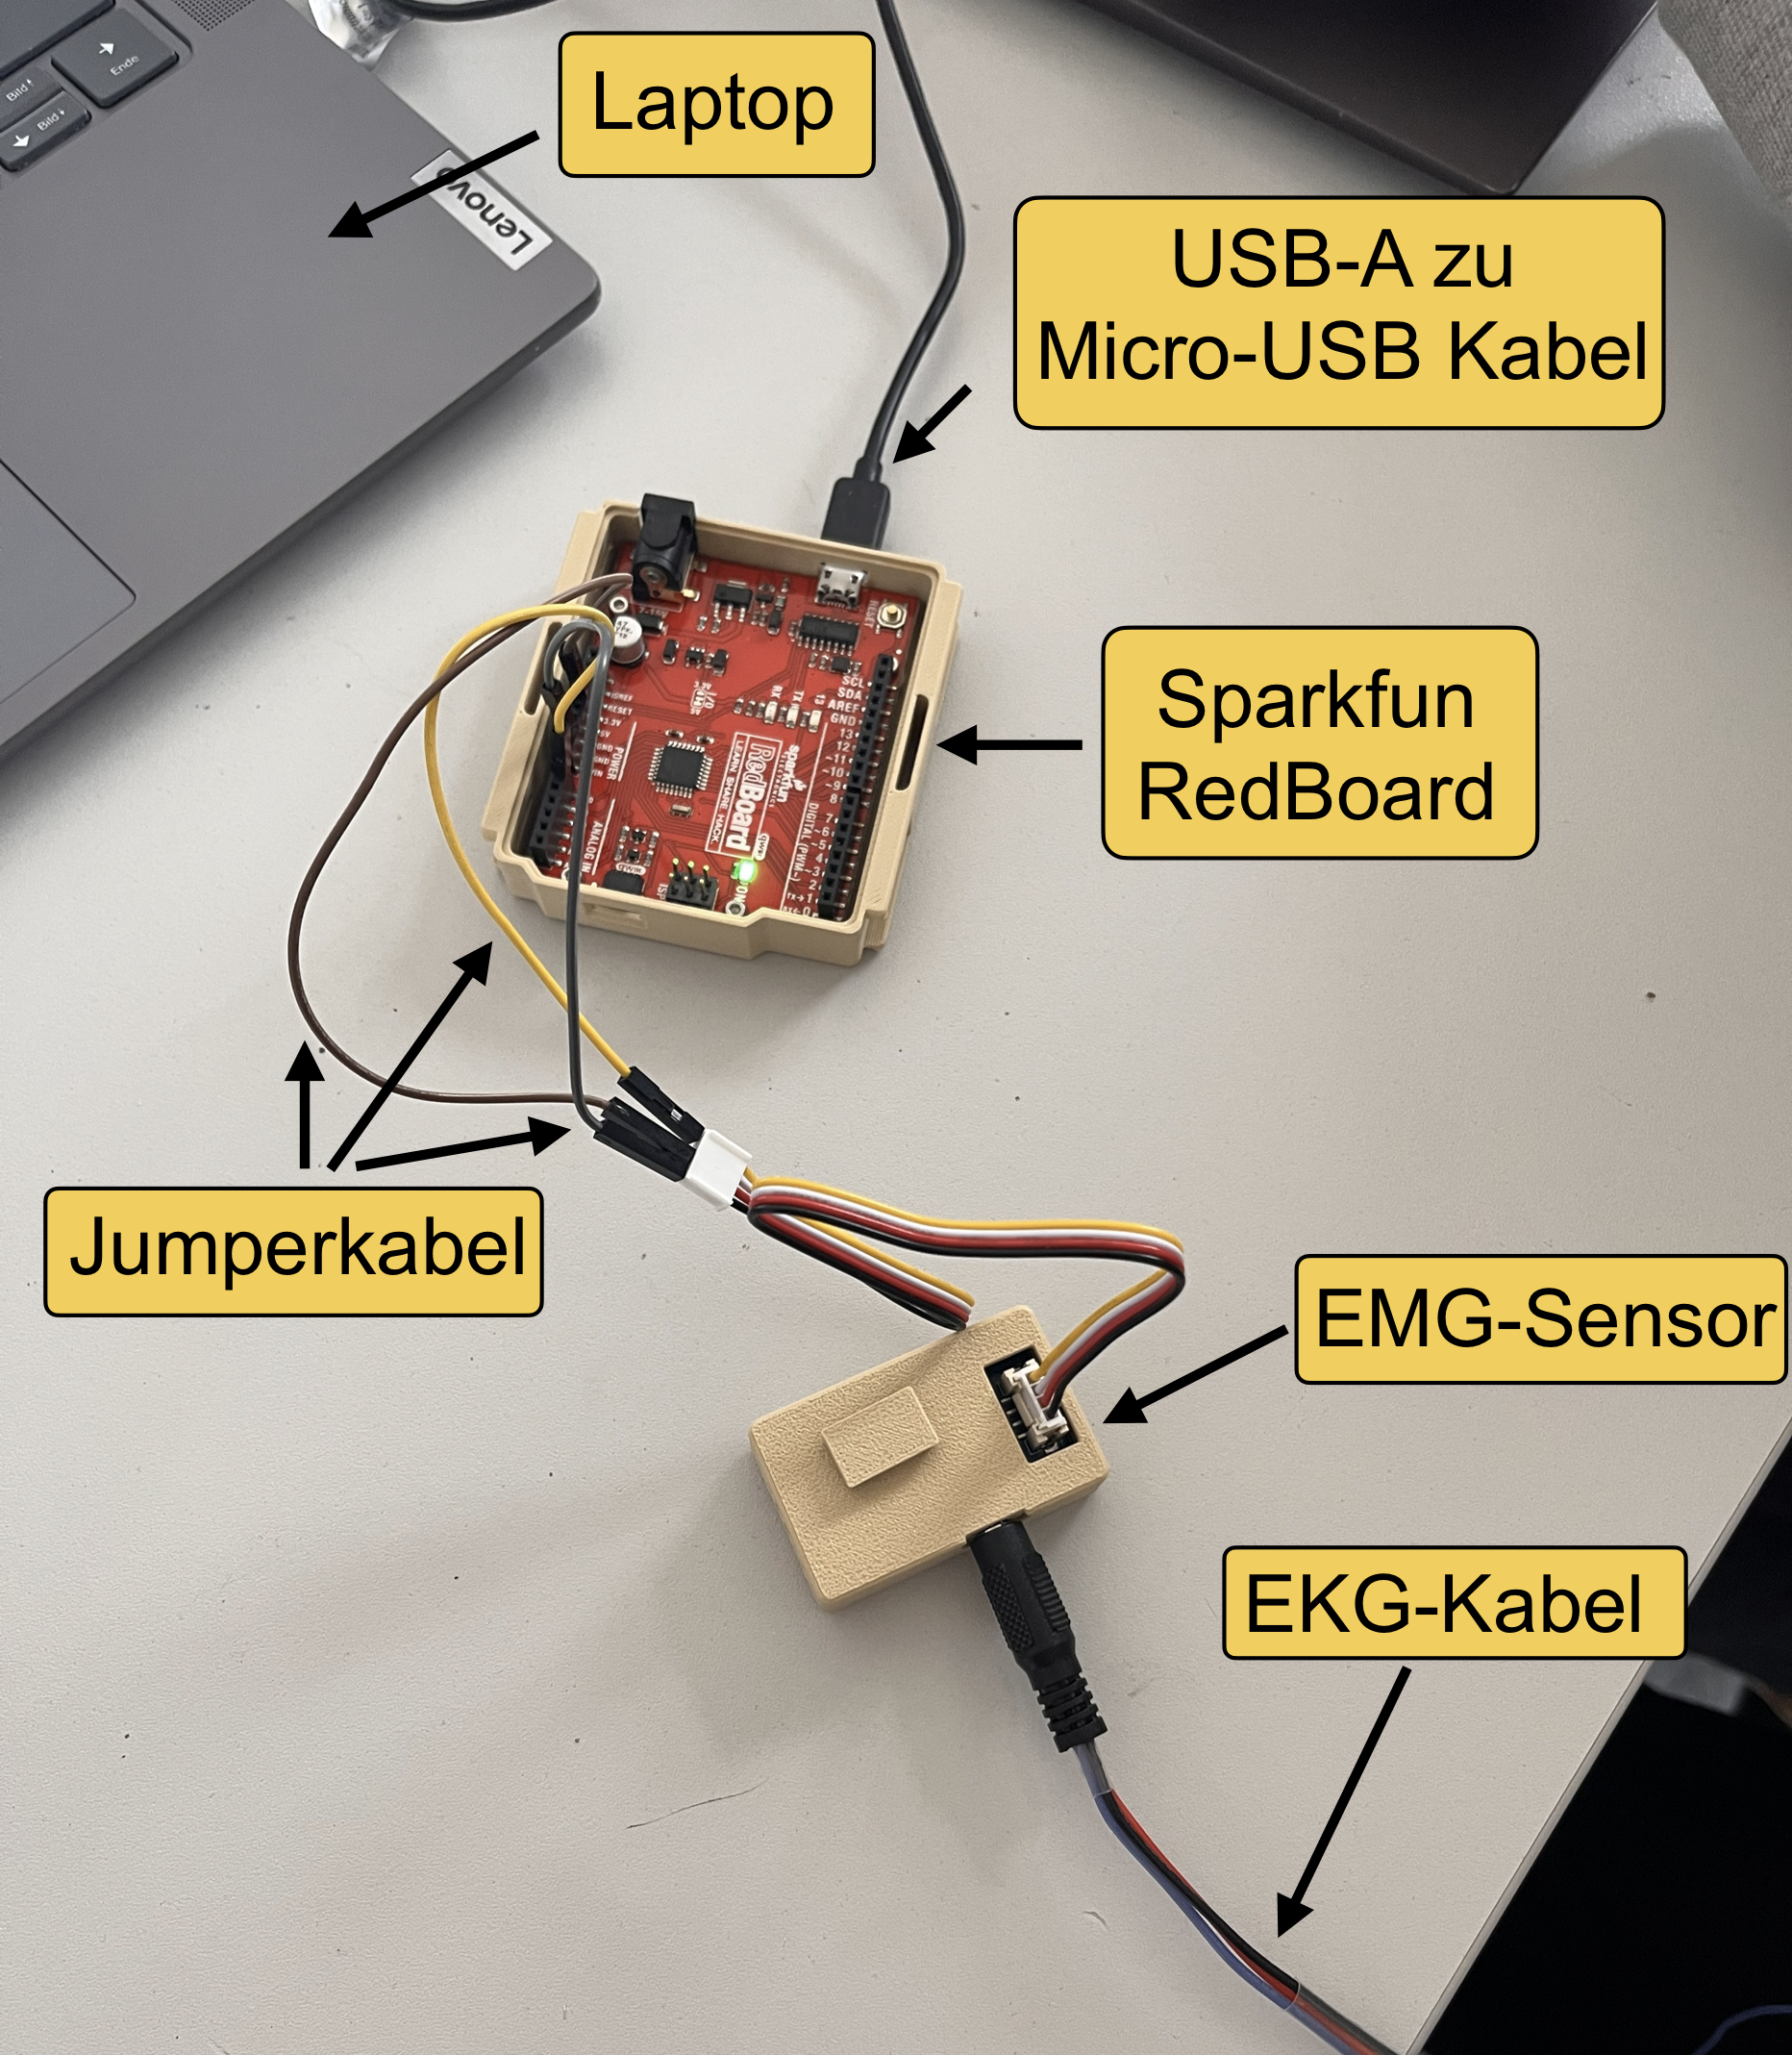
\includegraphics[width=0.4\textwidth]{figures/versuchsaufbau.png}
    \caption{Verbindung des EMG/EKG Sensors mit dem Sparkfun RedBoard Mikrocontroller}
    \label{fig:versuchsaufbau}
\end{figure}

\subsection*{Tabelle 1: Komponentenbeschreibungen}

\begin{table}[H]
    \centering
    \begin{tabular}{p{3.5cm} p{10cm}}
        \toprule
        Komponente & Beschreibung und Funktion \\
        \midrule
        EKG-Elektroden & Leitfähige Pads, die auf der Haut angebracht werden, um die biopotentiellen Spannungsdifferenzen des Herzens aufzunehmen und an das Sensorkabel weiterzuleiten. \\
        \midrule
        Sensormodul & Ein integrierter Signalaufbereitungsblock für EKG-Anwendungen. Er filtert Bewegungsartefakte und verstärkt das Millivolt-Signal auf einen für den Mikrocontroller lesbaren Pegel (0--3.3V oder 0--5V Output). \\
        \midrule
        SparkFun RedBoard (MCU) & Basiert auf dem ATmega328P Mikrocontroller (16 MHz). Er fungiert als ADC-Einheit, die das analoge Sensorsignal abtastet und digital verarbeitet. \\
        \midrule
        FTDI-Chip (Onboard) & Der FT231X Chip auf dem RedBoard wandelt die seriellen TTL-Signale des Mikrocontrollers in das USB-Protokoll um, damit der Computer diese lesen kann. \\
        \midrule
        Mini-USB Kabel & Physische Schnittstelle zur Übertragung der Daten vom FTDI-Chip zum PC sowie zur 5V-Stromversorgung des gesamten Boards. \\
        \midrule
        PC / Visualisierungssoftware & Empfängt den Datenstrom über den virtuellen COM-Port. Software (z.\,B. Serial Plotter oder Processing) stellt die Amplitudenwerte grafisch über der Zeit dar. \\
        \bottomrule
    \end{tabular}
    \label{tab:komponenten}
    \caption{Komponenten des EKG-Messsystems (Spezifikationen für SparkFun RedBoard).}
\end{table}

\subsection*{Tabelle 2: Signalpfade und Bussysteme}

\begin{table}[H]
    \centering
    \begin{tabular}{p{4cm} p{3cm} p{2.8cm} p{4cm}}
        \toprule
        Pfad / Verbindung &Bustyp / Signal & \textbf{Geschwindigkeit} & Technische Details \\
        \midrule
        Sensor $\rightarrow$ RedBoard Pin A0 & Analoges Spannungssignal & Kontinuierlich (Analog) & Übertragung der verstärkten Herzstromkurve als Spannungswert. \\
        \midrule
        Interne Verarbeitung (ATmega328P) & 10-Bit ADC Bus (Intern) & Abhängig vom Code (oft ca. 100-500 Hz Sampling) & Der interne ADC wandelt die Spannung in diskrete Integer-Werte von 0 bis 1023 um. \\
        \midrule
        ATmega328P $\rightarrow$ FTDI Chip & UART (TTL Seriell) & 500.000 Baud & Asynchrone serielle Übertragung über die RX/TX-Leitungen auf dem Board. \\
        \midrule
        RedBoard (USB) $\rightarrow$ PC & USB 2.0 (Virtual COM) & 12 Mbit/s (USB Full Speed) & Der FT231X Chip puffert die schnellen seriellen Daten und übergibt sie per USB an die Software. \\
        \bottomrule
    \end{tabular}
    \label{tab:signalpfade}
    \caption{Analyse der Signalpfade und Bus-Spezifikationen.}
\end{table}
\newpage

\subsection{Aufgabe 2: Daten im Seriellen Plotter}

\begin{figure}[h]
    \centering
    \includegraphics[width=0.7\textwidth]{figures/ecg_plots_with_and_without_charger.png}
    \caption{Serieller Plotter mit (oben) und ohne (unten) Netzanschluss}
    \label{fig:serial_plotter_noise_and_normal}
\end{figure}

Im seriellen Plotter wurden die Rohdaten des EKG-Signals visualisiert. Wie in Abbildung \ref{fig:serial_plotter_noise_and_normal} abgebildet konnte beobachtet werden,
dass, sobald der Laptop über ein Netzteil mit Strom versorgt wurde, starke Störungen in Form von Noise im Signal auftraten.
Diese Störung hat eine Frequenz von circa 50 Hz, weshalb davon auszugehen ist, dass es sich um Netzbrummen handelt.
Dies wurde durch die Verwendung des Laptops im Akkubetrieb vermieden. Alternativ wäre eine Filterung des Signals mit Tiefpassfiltern möglich gewesen.


\subsection{Aufgabe 3: Experiment in Ruhe}
\begin{figure}[h]
    \centering
    \includegraphics[width=0.7\textwidth]{figures/ecg_plots_all_participants.png}
    \caption{Rohdaten der Ruhe-EKGs für alle Teilnehmenden}
    \label{fig:ecg_plot_all_participants}
\end{figure}
In Abbildung \ref{fig:ecg_plot_all_participants} sind die Rohdaten der Ruhe-EKGs für alle Teilnehmenden für den Zeitraum von ca. 5 Sekunden (5000 ms) dargestellt.

\begin{figure}[h]
    \centering
    \includegraphics[width=0.7\textwidth]{figures/ecg_plot_Elias.png}
    \caption{EKG-Signal mit markierten P-, QRS- und T-Wellen für Elias}
    \label{fig:ecg_with_marked_waves_elias}
\end{figure}

In Abbildung \ref{fig:ecg_with_marked_waves_elias} ist das EKG-Signal von Elias mit den markierten P-(rot), QRS-(grün) und T-Wellen(gelb) dargestellt.
Die P-Welle repräsentiert die Depolarisation der Vorhöfe. Sie entsteht, wenn der elektrische Impuls vom Sinusknoten ausgeht und
sich über beide Vorhöfe ausbreitet. Dies führt zur Kontraktion der Vorhöfe und zum Bluttransport in die Herzkammern. Die P-Welle
ist normalerweise klein und positiv.
Der QRS-Komplex zeigt die Depolarisation der Herzkammern. Dieser scharfe, große Ausschlag entsteht, wenn sich der elektrische
Impuls vom AV-Knoten über das His-Bündel und die Purkinje-Fasern schnell durch die Ventrikel ausbreitet. Die resultierende Kontraktion der
Ventrikel pumpt das Blut in den Lungen- und Körperkreislauf. Der QRS-Komplex überlagert gleichzeitig die Repolarisation der Vorhöfe, die
dadurch im EKG nicht sichtbar ist.
Die T-Welle repräsentiert die Repolarisation der Ventrikel. Nach der Kontraktion kehren die Herzkammerzellen in ihren Ruhezustand zurück.
Dies bereitet das Herz auf den nächsten Zyklus vor. Die T-Welle ist
normalerweise positiv und breiter als der QRS-Komplex, da die Repolarisation langsamer abläuft als die Depolarisation.


\subsection{Aufgabe 4: Beschreibung und Erklärung des Ruhe-EKG Codes}
\subsubsection{Arduino Code}
Das bereitgestellte Skript Lab2Code1 \cite{Lab2Code1.ino} wurde verwendet, um die Rohdaten des EKG-Signals zu erfassen und über die serielle Schnittstelle an den Computer zu übertragen.
Von dort aus wurden die Daten im nachfolgenden Skript serialRead \cite{serialRead.ipynb} eingelesen und gespeichert, wie in Abschnitt \ref{sssec:PythonCode} beschrieben wird.
Der Code initialisiert die serielle Kommunikation mit einer Baudrate von 500000 und liest kontinuierlich die analogen Werte vom EKG-Sensor ein.
Dieser Wert wird dann nur an die Console weitergegeben, wenn eine Zeit von 1000 Millisekunden vergangen ist.
\subsubsection{Python Code}
\label{sssec:PythonCode}
Der Code serialRead \cite{serialRead.ipynb} wurde ebenfalls bereitgestellt. 
In diesem Skript können die serielle Schnittstelle, die Baudrate und die Dauer der Aufnahme sowie der Name des Outputdokuments als Variablen gesetzt werden.
Die Funktion sampling() öffnet die serielle Schnittstelle und das Outputdkoument und liest dann die Daten für die angegebene Dauer ein.
Die eingelesenen Daten werden in eine Liste gespeichert und anschließend in das Outputdokument geschrieben.
Danach werden Informationen zur gemittelten Samplingrate über die gesamte Aufnahmezeit, totale Anzahl an Samples und vergangener Zeit sowie der Speicherbestätigung ausgegeben.
Die Funktion gibt den Wert der errechneten Sampling Rate zurück.
Im zweiten Teil des Codes werden die Daten aus dem Outputdokument eingelesen und in einem Plot visualisiert, um direkt die Qualität der Aufnahme beurteilen zu können.

\subsection{Aufgabe 5: Fünf-Sekunden-Plot der Ruhe-EKGs}

\begin{figure}[h]
    \centering
    \includegraphics[width=0.7\textwidth]{figures/ecg_with_rwaves_Elias.png}
    \caption{EKG-Signal mit markierten R-Zacken für Elias}
    \label{fig:ecg_with_rwaves_elias}
\end{figure}    

Abbildung \ref{fig:ecg_with_rwaves_elias} zeigt das EKG-Signal von Elias mit den markierten R-Zacken in einem ausgesuchten Bereich mit ca. 5 Sekunden Länge.
Die Positionen der R-Zacken wurden durch die gebenen Funktionen in Lab2Functions.py \cite{Lab2Functions.py} berechnet und anschließend in dem Plot dargestellt.
\subsection{Aufgabe 6: Errechnete Daten der Ruhe-EKGs}

\begin{table}[h]
    \centering
    \begin{tabularx}{\textwidth}{l l X}
        \hline
        \textbf{Teilnehmer} & \textbf{Herzfrequenzvariabilität} & \textbf{mittlere Herzfrequenz} \\
        \hline
        Hauke & 113.35 & 60.21 \\
        Lasse & 57.51 & 73.44 \\
        Elias & 83.23 & 68.04 \\
        \hline
    \end{tabularx}
    \caption[Herzfrequenzvariabilität und Herzfrequenz]{Die errechnete Herzfrequenzvariabilität (in ms) und Herzfrequenz (in bpm) für alle Teilnehmenden}
    \label{tab:vergleich_errechnete_hrv_und_hr}
\end{table}

In Tabelle \ref{tab:vergleich_errechnete_hrv_und_hr} sind die errechneten Werte für die Herzfrequenzvariabilität (in ms) und die Herzfrequenz (in bpm) für alle Teilnehmenden dargestellt.
Die Herzfrequenzvariabilität wurde als Standardabweichung der RR-Intervalle berechnet, während die Herzfrequenz aus der durchschnittlichen Anzahl der Herzschläge pro Minute abgeleitet wurde.
Wie in der Tabelle zu sehen ist, sind die Unterschiede zwischen den Teilnehmenden sowohl in der Herzfrequenzvariabilität als auch in der Herzfrequenz deutlich erkennbar. Die Ursachen für diese
Unterschiede können von individuellen physiologischen Faktoren und von externen Messbedingungen (bspw. lose sitzende Elektroden) abhängen. 


\subsection{Aufgabe 7: Einordnung der Daten im Kontext derer der Mitstudierenden}
Im Histogramm zur Verteilung der Herzfrequenzen \ref{fig:histogram_herzfrequenz} zeigt sich, dass die mittlere Herzfrequenz bei Frauen und Männern ähnlich verteilt ist,
wobei beide Geschlechter einen Mittelwert um 63-65 bpm aufweisen.
\begin{figure}[h]
    \centering
    \includegraphics[width=0.5\textwidth]{figures/Histogramm_Herzfrequenz.png}
    \caption{Histogramm der Herzfrequenzverteilung nach Geschlecht}
    \label{fig:histogram_herzfrequenz}
\end{figure}

Im Histogramm zur Herzfrequenzvariabilität \ref{fig:histogram_hfv} ist eine größere Streuung erkennbar,
wobei beide Geschlechter eine breite Verteilung zeigen.
\begin{figure}[h]
    \centering
    \includegraphics[width=0.5\textwidth]{figures/Histogramm_HFV.png}
    \caption{Histogramm der Herzfrequenzvariabilität nach Geschlecht}
    \label{fig:histogram_hfv}
\end{figure}
Die Daten der Mitstudierenden wurden aus dem geteilten Google Sheet \cite{GoogleSheetHRKurs} entnommen und leicht angepasst, da eindeutig Tippfehler eingebaut wurden.
Für beide Histogramm lässt sich sagen, dass die großen Überlappungen zwischen den Geschlechtern darauf hindeuten,
dass die interindividuelle Variabilität größer ist als geschlechtsspezifische Unterschiede sind. Mögliche Ursachen für nicht erkennbare 
Geschlechtsunterschiede könnten die relativ kleine Stichprobengröße, ähnliche Fitnesslevel der Teilnehmenden oder unterschiedliche
Messbedingungen sein.
\newline
Unsere Werte für die Herzfrequenz und die Herzfrequenzvariabilität liegen im erwarteten Bereich für gesunde Erwachsene in Ruhe.
Auch im direkten Vergleich mit den Werten der Mitstudierenden wird deutlich, dass sich unsere Werte im ähnlichen Bereich bewegen.
Generell ist wichtig zu erwähnen, dass sich viele sehr fitte Personen in der Gruppe befinden, was die tendenziell niedrigeren Herzfrequenzen
erklären könnte. Außer der Tatsache, dass die Variabilität der Herzfrequenzen bei einigen Anderen als auch bei Hauke höher ist, als die, 
die normalerweise für gesunde Erwachsene erwartet werden. Das lässt auf eine etwas ungenaue Messung oder Bewegungsartefakte schließen.
\newline
Die Literatur gibt für die Ruhe-Herzfrequenz bei gesunden Erwachsenen einen Normalbereich von 60-100 bpm an, wobei der Durchschnitt bei etwa
70-75 bpm liegt. Gut trainierte Personen können Werte von 40-60 bpm aufweisen. Die Klassendaten zeigen ohne Berücksichtigung der extremen
Ausreißer bei Frauen einen Mittelwert von etwa 62-65 bpm und bei Männern von etwa 63-67 bpm, mit einem Gesamtbereich von circa 42-89 bpm.
Diese Werte liegen größtenteils im normalen bis niedrig-normalen Bereich. Die Frage, ob es sich wirklich um ruhende Herzfrequenzen handelt,
lässt sich nicht eindeutig mit Ja oder Nein beantworten. Einerseits sprechen die Werte im Bereich von 50-70 bpm für echte Ruhebedingungen,
insbesondere bei den Messungen in liegender Position. Andererseits deuten Werte über 75-80 bpm auf erhöhte Herzfrequenzen hin, die nicht
mehr als echte Ruhe betrachtet werden können. Die sitzenden Messungen führen bereits zu einer höheren Grundfrequenz. Auch die Messsituation
selbst kann bei einigen Probanden zu Stress oder Aufregung geführt haben. Die relativ hohe Streuung der Werte innerhalb der
Klasse deutet darauf hin, dass unterschiedliche Messbedingungen und individuelle Reaktionen vorlagen. Zusammenfassend lässt sich sagen,
dass die Verteilung der Herzfrequenzen in der Klasse eine Mischung aus echten Ruhewerten und erhöhten Werten darstellt. Für standardisierte
Messungen der Ruhe-Herzfrequenz wären ausschließlich liegende, störungsfreie Bedingungen über mehrere Minuten ideal gewesen.

\subsection{Aufgabe 8: Plot der Herzfrequenz während des Belastungs-EKGs}
\begin{figure}[h]
    \centering
    \includegraphics[width=0.7\textwidth]{figures/windowed_hr.png}
    \caption{Herzfrequenz während des Belastungs-EKGs}
    \label{fig:heart_rate_belastung}
\end{figure}
In Abbildung \ref{fig:heart_rate_belastung} ist die Herzfrequenz über der Zeit während des Belastungs-EKGs dargestellt. Die drei Phasen Ruhe,
Belastung und Erholung sind klar erkennbar und zeigen die erwarteten Veränderungen der Herzfrequenz in Reaktion auf körperliche Aktivität.
In den folgende Abschnitten werden die einzelnen Phasen genauer analysiert.

\subsection{Aufgabe 9: Ruhephase vor Belastungs-EKG}
Die Herzfrequenz steigt bei körperlicher Belastung nicht sofort an, sondern folgt einer charakteristischen Dynamik. Unmittelbar zu Beginn 
der Übung zeigt sich eine kurze Verzögerungsphase von etwa 5 bis 10 Sekunden, in der die Herzfrequenz noch nahezu auf Ruheniveau verbleibt. 
Anschließend folgt eine schnelle Anstiegsphase, in der die Herzfrequenz rasch zunimmt. Bei konstanter Belastung erreicht die Herzfrequenz 
nach etwa 2 bis 3 Minuten ein Plateau, das der Belastungsintensität entspricht. Start der Übung und Anstieg der Herzfrequenz fallen nicht 
zeitgleich zusammen, weil mehrere physiologische Prozesse ablaufen müssen. Mechanische und chemische Rezeptoren in den Muskeln müssen die 
erhöhte Aktivität registrieren und Signale an das Herz-Kreislauf-Zentrum senden.
\newline
Unter Cardiac Output, auch Herzzeitvolumen genannt, versteht man das Blutvolumen, das vom Herzen pro Minute in den Kreislauf gepumpt wird. 
Er berechnet sich aus dem Produkt von Herzfrequenz und Schlagvolumen und beträgt beim gesunden Erwachsenen in Ruhe etwa 5 Liter pro Minute. 
Eine plötzliche Aktivierung der Muskulatur bewirkt keine direkte Änderung des Cardiac Outputs, weil beide Komponenten, aus denen er sich 
zusammensetzt, nicht instantan reagieren können. Somit steigt der Cardiac Output erst verzögert an, sobald sowohl die Herzfrequenz als auch das 
Schlagvolumen auf die erhöhten metabolischen Anforderungen reagiert haben.
\begin{figure}[h]
    \centering
    \includegraphics[width=0.7\textwidth]{figures/windowed_hr_with_averages.png}
    \caption{Herzfrequenz mit markierten Phasen (Ruhe, Belastung, Erholung) und Durchschnittswerten.}
    \label{fig:hr_with_averages1}
\end{figure}

\subsection{Aufgabe 10: Erholungsphase nach Belastungs-EKG}
Ja, die Herzfrequenz kehrt nach Ende der Belastung zum ursprünglichen Ruhepuls zurück. 
Dieser Prozess dauert in der Regel zwischen 3 und 10 Minuten, abhängig von der Belastungsintensität, der Belastungsdauer und dem 
individuellen Trainingszustand.
Dieser Prozess dauert relativ lange, weil mehrere physiologische Mechanismen ablaufen müssen. Das sympathische Nervensystem, 
das während der Belastung aktiviert wurde, muss herunterreguliert werden, während gleichzeitig der parasympathische Tonus wieder zunimmt. 
Dieser autonome Umschaltprozess benötigt Zeit. Zudem muss der Körper metabolische Prozesse abschließen, wie die Rückzahlung der 
Sauerstoffschuld und die Beseitigung von Stoffwechselprodukten wie Laktat. Die erhöhte Körpertemperatur nach Belastung hält die 
Herzfrequenz ebenfalls vorübergehend erhöht, da das Herz-Kreislauf-System zur Wärmeabgabe beiträgt.
\newline
Die Zeit bis zur Rückkehr zum Ruhepuls ist unterschiedlich je nach Trainingszustand. Gut trainierte Personen zeigen in der Regel eine 
schnellere Erholung der Herzfrequenz, da ihr Herz-Kreislauf-System effizienter arbeitet, diese Abläufe häufiger durchmacht und somit 
schneller auf Ruhebedingungen umschalten kann.

\subsection{Aufgabe 11: Berechnen des metabolischen Energieverbrauchs}

%In der Funktion \texttt{analyze_ecg_and_plot()} aus der Datei \ref{analyzeHearthdata} wurde die Formel zur Berechnung des Energieverbrauchs 
%aus Model 1 für Männer aus dem Paper \cite{Hiilloskorpi2003HeartRateEnergyExpenditure} implementiert.
%\newline
%In Abbildung \ref{fig:energy_expenditure_belastung.png} ist der berechnete Energieverbrauch während des Belastungs-EKGs dargestellt.
%Darin ist wie erwartet zu erkennen, dass der Energieverbrauch während der Belastungsphase deutlich ansteigt und in in der Erholungsphase 
%wieder abfällt, allerdings nicht sofort auf das Ruhe-Niveau. Der Energieverbauch ist direkt an die Herzfrequenz gekoppelt, weshalb die 
%Annäherung des Models an die erwarteten Werte recht gut ist, da intuitiv mit steigender Belastung auch der Energieverbrauch steigt. Dieser 
%Trend ist in der Abbildung \ref{fig:energy_expenditure_belastung.png} klar erkennbar.
%\begin{figure}[h]
%    \centering
%    \includegraphics[width=0.7\textwidth]{figures/Energieverbrauch_Belastung.png}
%    \caption{Berechneter Energieverbrauch während des Belastungs-EKGs}
%    \label{fig:energy_expenditure_belastung.png}
%\end{figure}

\subsection{Aufgabe 12: Einordnung des Energieverbrauchs und entsprechender Code}
Der gesamte Energieverbrauch über das Belasungs-EKG beträgt circa \newline
-> HIER WERT EINFÜGEN <- \newline
\begin{table}[ht]
    \centering
    \begin{tabularx}{\textwidth}{l l}
        \hline
        Menge & Energieeinheit \\
        \hline
        Zahl1 & Joule \\
        Zahl2 & Kalorien \\
        zahl3 & Rittersporttafeln \\
        Zahl4 & Bier \\
        Zahl5 & Anteil des Kalorienbedarfs von Lasse \\
        \hline
    \end{tabularx}
    \caption[Aufgabe 12]{Umgerechneter Energieverbrauch während des Belastungs-EKGs}
    \label{tab:umgerechneterEnergieverbrauch}
\end{table}
Das entspricht ungefähr den in Tabelle \ref{tab:umgerechneterEnergieverbrauch} umgerechneten Einheiten.
Die Werte wurden mit der Funktion \texttt{calculateenergy()} aus der Datei \cite{calculateEnergy} berechnet.

